\documentclass[a4paper, openany]{memoir}

\usepackage[utf8]{inputenc}
\usepackage[T1]{fontenc} 
\usepackage[english]{babel}

\usepackage{fancyhdr}
\usepackage{float}

\usepackage{amsmath}
\usepackage{amsthm}
\usepackage{amssymb}
\usepackage{enumitem}
\usepackage{multicol}
\usepackage[bookmarksopen=true,bookmarksopenlevel=2]{hyperref}
\usepackage{tikz}
\usepackage{indentfirst}

\pagestyle{fancy}
\fancyhf{}
\fancyhead[LE]{\leftmark}
\fancyhead[RO]{\rightmark}
\fancyhead[RE, LO]{Data Fundamentals}
\fancyfoot[LE, RO]{\thepage}
\fancyfoot[RE, LO]{Pete Gautam}

\renewcommand{\headrulewidth}{1.5pt}

\chapterstyle{thatcher}
\begin{document}
    \chapter{Numerical Arrays}
    \section{ndarrays}
    In this course, the data type we shall be focusing on is multi-dimensional numerical arrays. They are called ndarrays (for $n$-dimensional arrays). Arrays can be used to represent various types of data, e.g. sound, image, video, tabular data, etc.

    Multi-dimensional arrays can be easily manipulated with vectorised operations. These are operations that we apply on an entire array without explicitly writing the loop. For example, assume that we have the array \texttt{pos}, containing 100 2D coordinates. If we wanted to scale the coordinates by 2 and add an offset of 10 in the $y$-value, we could simply write \texttt{pos = pos * 2 + [0, 10]}. There are no explicit loops, which makes the operations much clearer to read and understand.

    In particular, vectorisation is a special type of parallel computing, where the arrays are restricted to a particular size. Modern CPUs have vectorised operations to perform the same task on multiple elements at once (i.e. one clock cycle)- this is called single instruction multiple data (SIMD). GPUs can perform calculations much faster than a CPU.

    \subsection{Shapes of arrays}
    ndarrays have dimensions (or ranks). A 1D array is a vector. A 2D array is a matrix. An array of higher dimension is called a tensor. The shape of an array refers to the number of elements it can hold in each dimension.

    We refer to each dimension within an array by axis. This is indexed by 0, i.e. axis 0 is the rows; axis 1 is the columns; and axis 2 is the depth/frames/etc.

    \subsection{Array operations}
    There are many types of operations that we can perform on array(s), such as:
    \begin{itemize}
        \item arithmetic, e.g. addition and subtraction;
        \item indexing and slicing;
        \item generating arrays, e.g. an array with uniformly distributed numbers between 0 and 1;
        \item rearranging arrays, e.g. taking the transpose of a matrix or reshaping the array;
        \item ordering arrays, e.g. sorting the array; and
        \item aggregation, e.g. finding the sum, start and stop.
    \end{itemize}

    \subsection{Static arrays}
    There are many differences between a list and an ndarray, as highlighted below:
    \begin{itemize}
        \item ndarrays have a fixed, pre-defined size (or shape). They cannot be extended/resized after definition.
        \item ndarrays have a fixed, pre-defined type.
        \item ndarrays can only hold numbers (usually).
        \item ndarrays are meant to hold multi-dimensional data.
        \item ndarrays must be rectangular in shape, e.g. equal number of rows in each column.
    \end{itemize}
    Nonetheless, ndarrays are still mutable, e.g. we can set a value of the array without creating a new copy.

    When initialising ndarrays, we need to specify its type. This is because an ndarray is stored as a block of raw numbers. For this reason, ndarrays have a thin wrapper raw blocks of memory. As a result, they are much more efficiently stored and operations can be performed on them must faster.
    \newpage

    \section{NumPy}
    We will be using NumPy, which contains a class for ndarrays. An array in NumPy has:
    \begin{itemize}
        \item a shape (e.g. \texttt{(5, 6)}) and
        \item a dtype (e.g. \texttt{float64}).
    \end{itemize}

    Given a list, we can convert it into an array using \texttt{np.array(list)}. We can also create an array in NumPy in the following ways:
    \begin{itemize}
        \item \texttt{np.empty(shape)}- it allocates space for an array of the given shape;
        \item \texttt{np.zeros(shape)}- it initialises an array of the given shape with zeroes everywhere;
        \item \texttt{np.ones(shape)}- it initialises an array of the given shape with ones everywhere;
        \item \texttt{np.full(shape, value)}- it initialises an array of the given shape with the given value everywhere.
    \end{itemize}
    All the functions that initialise an array first call \texttt{np.empty(shape)} to allocate the space. The functions above also have a `like' version, where instead of providing the shape, we provide an array and take its shape, e.g. \texttt{np.ones\_like(array)}.

    We can also create arrays with random entries given below:
    \begin{itemize}
        \item \texttt{np.random.randint(start, stop, shape)}- creates an array with uniform random integers between the given start (inclusive) and the given stop (exclusive);
        \item \texttt{np.random.uniform(start, stop, shape)}- creates an array with uniform random floating point numbers between the given stop and start;
        \item \texttt{np.random.normal(mu, sigma, shape)}- creates an array with normally distributed random floating point numbers with the mean mu, and standard deviation sigma;
    \end{itemize}
    We can also create a range of numbers:
    \begin{itemize}
        \item \texttt{np.arange(value)}- creates a 1D array of numbers from 0 (inclusive) to value (exlusive);
        \item \texttt{np.arange(start, stop)}- creates a 1D array of numbers from start (inclusive) to stop (exclusive);
        \item \texttt{np.arange(start, stop, step)}- creates a 1D array of numbers from start (inclusive) to end (exclusive), with the given step;
        \item \texttt{np.linspace(start, stop, step)}- creates a 1D array of numbers from start (inclusive) to stop (inclusive), with the given step.
    \end{itemize}

    We can open a text file using \texttt{np.loadtxt(fname)} and save a file using \texttt{np.savetxt(array, fname)}.

    \subsection{Slicing and indexing}
    Indexing is taking an element from the array, while slicing is taking a subset of the array. We take the multi-dimensional indices when indexing. We have 3 parameters in slicing- \texttt{start}, \texttt{stop} and \texttt{step}, like in vanilla Python. We can reverse an array by using step size -1.

    Slicing does not change the rank of an array- it selects a rectangular subset with the same number of dimensions. On the other hand, indexing (usually) reduces the rank- it selects a rectangular subset where one dimension is a singleton.

    We can also transpose an array- this exchanges the rows and columns for a 2D array, and flips the order of the axes in general. It is given by \texttt{array.T}. This operation takes $O(1)$ time.

    \subsection{Concatenation and Stacking}
    We can join two arrays (concatenation), or create a new array with the two arrays (stacking). The arrays must be of the right shape for this to happen. If we are concatenating with multiple dimensions, the axis of concatenation must be specified.

    \subsection{Tiling}
    We can repeat an array multiple times. The function \texttt{np.tile(array, lines)} returns another array where the shape of the tiling states how the array should be repeated/joined.

    \subsection{Boolean Arrays} Using boolean arrays, we can check whether elements in the array satisfy a condition. Using the condition \texttt{np.where(bool, a, b)}, we create another array, where \texttt{a} is what the value of something that satisfies the condition, and \texttt{b} is what the value of something that doesn't satisfy the condition. Using \texttt{np.nonzero(bool)}, we get an array of indices whether the value is true. We can generate boolean arrays by comparing two arrays, e.g. \texttt{x < y}.
    \newpage

    \section{Map and broadcast}
    \subsection{Maps}
    We can apply a function to each element within an array- this is elementwise computation. A map operation can have:
    \begin{itemize}
        \item single argument, e.g. \texttt{np.tan(x)} or \texttt{-x};
        \item two arguments, e.g. \texttt{x-y} or \texttt{np.maximum(x, y)}; or
        \item something else, e.g. \texttt{np.where(x, 0, 1)}.
    \end{itemize}

    In a map operation with multiple arrays, their shapes must be compatible. If the two arrays have the same shape, then the operations is applied elementwise. Otherwise, one of the arrays will be broadcasted so that they have the same shape. Broadcasting involves tiling one of the arrays until the two arrays have the same shape, if possible. This is much more efficient than explicit broadcasting.

    \subsection{Broadcasting}
    Broadcasting is how arithmetic operations are done on arrays which have different shapes. The rules are:
    \begin{itemize}
        \item If the two arrays have the same number of dimensions, then they must have the same shape. The operation is done elementwise.
        \item If one array has fewer dimensions than the other, then the last dimensions of the bigger array must match the dimensions of the smaller array.
    \end{itemize}
    For example,
    \begin{itemize}
        \item \texttt{shape(2, 2) * shape(2, 2)} is allowed;
        \item \texttt{shape(2, 3, 4) * shape(3, 4)} is allowed;
        \item \texttt{shape(2, 3, 4) * shape(2, 3)} is not allowed.
    \end{itemize}
    To perform the operation column-wise, we can transpose, perform the operation, then transpose back.
    \newpage

    \section{Reduction and accumulation}
    \subsection{Reduction}
    A reduction/aggregation applies a function to two elements within the array repeatedly to return a scalar. These operations are:
    \begin{itemize}
        \item \texttt{np.all(array)} combines the elements in the (boolean) array with \texttt{AND};
        \item \texttt{np.any(array)} combines the elements in the (boolean) array with \texttt{OR};
        \item \texttt{np.min(array)} combines the elements in the array with the minimum operation;
        \item \texttt{np.max(array)} combines the elements in the array with the maximum operation;
        \item \texttt{np.sum(array)} combines the elements in the array with \texttt{+};
        \item \texttt{np.prod(array)} combines the elements in the array with \texttt{*};
        \item \texttt{np.mean(array)} calls \texttt{np.sum(array)} and then divides the result by \texttt{len(array)};
        \item \texttt{np.std(array)} calls \texttt{np.mean(array)} and then applies the standard deviation formula.
    \end{itemize}
    We can specify the axis/axes to only reduce with respect to the given dimension(s). By default, it reduces with respect to all the axes.

    \subsection{Accumulation}
    Accumulative is the cumulative sum/product of the array. The operations are:
    \begin{itemize}
        \item \texttt{np.cumsum(array)} is the accumulation of \texttt{+};
        \item \texttt{np.cumprod(array)} is the accumulation of \texttt{*};
        \item \texttt{np.diff(array)} is the accumulation of \texttt{-} and has one less output than input;
        \item \texttt{np.gradient(array)} is like \texttt{np.diff(array)}, but uses central differences to get the same length output, and it computes the gradient over every axis and returns them all in a list.
    \end{itemize}

    \subsection{Finding}
    We can find the indices that match the given criteria:
    \begin{itemize}
        \item \texttt{np.argmax(array)} returns the index of the maximum element in the array;
        \item \texttt{np.argmin(array)} returns the the index of the minimum element of the array;
        \item \texttt{np.argsort(array)} returns the indices of tthe elements in the array such that those indices represent the array sorted (we can index the array using the argsorted array to get the sorted array- this is fancy indexing);
        \item \texttt{np.nonzero(array)} returns the indices of all the non-zero elements in the array (or \texttt{True} in boolean arrays).
    \end{itemize}
    \newpage

    \section{Introduction to floating point}
    There are various representations of numbers. The two main classes of numbers are integers and floats. The ranges of different data types is given below.
    \begin{figure}[H]
        \centering
        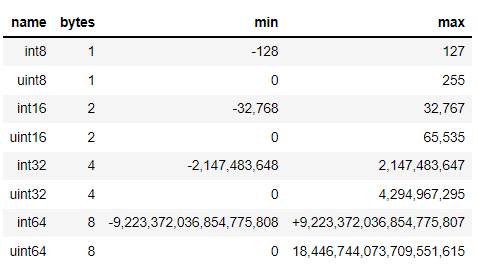
\includegraphics[scale=0.9]{src/1.1 ranges for different types.PNG}
        \caption{Ranges for different data types}
    \end{figure}
    \noindent If we apply an operation that exceeds that maximum value, then we have overflow. Overflows have undefined behaviour. Also, the order of operation matters in code, so some algebraic properties are lost, especially if the numbers are really different. For example, it might be that $ab \neq ba$, $a + b \neq b + a$, and so on.
    
    Floating point numbers can represent a much bigger range of numbers. To acheive this, they store:
    \begin{itemize}
        \item the mantissa- a fractional number with a standardised range (a number from 1.0 to just less than 2.0); and
        \item the exponent- a scaling or stretching factor (powers of 2).
    \end{itemize}
    Using this representation, we can store a lot of digits with very few values. They are, however, less precise than integers for this reason- numbers close to 0 can be represented quite precisely, but big numbers cannot be represented with such precision. A floating point number also stores the sign- whether the number is positive or negative.

    A floating point number can therefore be constructed using the three parts. In particular,
    \[\texttt{value} = \texttt{sign} * (1.\texttt{[mantissa]}) * (2^{\texttt{exponent}}).\]
    Since the value before the mantissa is always 1, we do not need to store it explictly. For example, the \texttt{float32} format of a number is:
    \begin{itemize}
        \item 1 bit for the sign;
        \item 8 bits for the exponent; and
        \item the remaining 23 bits for the mantissa.
    \end{itemize}
    In binary, a \texttt{float64} format is:
    \[\texttt{1} \qquad \texttt{10000011} \qquad \texttt{00100111010001001000101}.\]
    Here,
    \begin{itemize}
        \item the number is negative, since the sign is 1;
        \item the mantissa represents \texttt{1.00100111010001001000101}. In decimal, this is \texttt{1.153389573097229};
        \item the exponent represents $2^{131 - 127} = 2^4 = 16$ since $10000011_2 = 131_{10}$. We subtract 127 because of the implied offset.
    \end{itemize}
    Therefore, the number is $-18.454233169555664$.

    The standard for floating point numbers is IEEE754, which specifies the representation of floats, operations on them and some ``special'' numbers. The standards are given below:
    \begin{figure}[H]
        \centering
        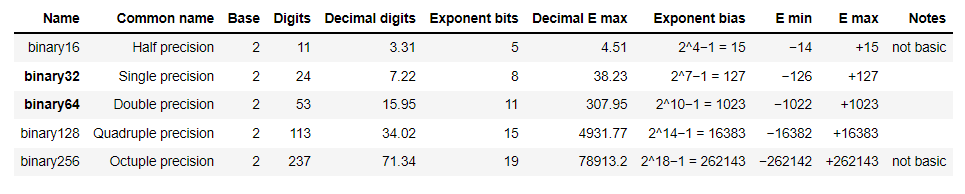
\includegraphics[scale=0.55]{src/1.2 IEEE754 standards.PNG}
        \caption{IEEE754 standards}
    \end{figure}
    Most of the time, we will be using either single precision \texttt{float32} (float) or double precision \texttt{float64} (double). GPUs typically are fastest (by a long way) using \texttt{float32}, but can do double precision \texttt{float64} computations at some significant cost. Most desktop CPUs (e.g. x86) have specialised float64 hardware.

    \subsection{Binary representation of floats}
    We will now look at some float representations.
    \begin{itemize}
        \item The float representation for 1 is
        \[\texttt{0} \qquad \texttt{01111111111} \qquad \texttt{00..00}\]
        The sign bit is 0, so the number is positive. The exponent is 0 (after subtracting the bias), and the mantissa is all 0s. So, the value is $2^0$.

        \item The float representation for 4 is
        \[\texttt{0} \qquad \texttt{10000000001} \qquad \texttt{00..00}\]
        Here, the exponent is 2 and the mantissa is all 0s- the value is $2^2$.
        
        \item The float representation for 5 is
        \[\texttt{0} \qquad \texttt{10000000001} \qquad \texttt{0100..00}\]
        Here, the exponent is 2, and the mantissa is 1.25. So, the value is $2^2 \cdot 1.25$.

        \item The float representation for 0.25 is
        \[\texttt{0} \qquad \texttt{01111111101} \qquad \texttt{00..00}\]
        Here, the exponent is $-2$, and the mantissa is all 0s- the value is $2^{-2}$.

        \item The float representation for 1/3 is
        \[\texttt{0} \qquad \texttt{01111111101} \qquad \texttt{01..01}\]
        Here, the exponent is $-2$, and the mantissa is $1.33333\dots$. So, the value is $2^{-2} * 1.33$. This number isn't represented exactly in binary.

        \item The float representation for 2000000.01 is
        \[\texttt{0} \qquad \texttt{10000010011} \qquad \texttt{111010000100100....00101001}\]
        This number also cannot be represented exactly.

        \item The float representation for 1e-90 is
        \[\texttt{0} \qquad \texttt{01011010100} \qquad \texttt{0000010010111101....11001101111}\]
        This number can be represented precisely.

        \item The float representation for 1.5e300 is
        \[\texttt{0} \qquad \texttt{11111100100} \qquad \texttt{000111101011001....0000110101}\]        This number cannot be represented precisely- we represent the value with the closest number to it.
    \end{itemize}

    In float64, every integer from $-2^{53}$ to $2^{53}$ can be represented precisely; integers outside of this range are not represented exactly. This is because the mantissa has 53 bits.
    \newpage

    \section{Floating point weirdness}
    There are 5 types of errors with floats:
    \begin{itemize}
        \item Invalid operations- this occurs when the result of the operation is not a real number/undefined, e.g. \texttt{0/0} or \texttt{sqrt(-1)};
        \item Division by zero- this occurs when dividing a (nonzero) number by 0;
        \item Overflow- this occurs if the result of a computation exceeds the limits of the floating point number;
        \item Underflow- this occurs if the result of a computation is smaller than the smallest representable number, and so is rounded off to zero;
        \item Inexact- this occurs if a computation will produce an inexact result due to rounding.
    \end{itemize}

    An exception might be trapped or untrapped. An untrapped exception will not halt execution, and will instead do some default operation (e.g. untrapped divide by zero will output \texttt{np.inf} instead of halting). A trapped exception will cause the process to be signalled in to indicate that the operation is problematic, at which point it can either halt or take another action. Typically, invalid operation is trapped; inexact and underflow aren't trapped; and division by zero and overflow might or might not trapped. It is possible to manually trap them.

    There are 2 versions of 0- $+0$ and $-0$. The \texttt{float64} representation of $+0.0$ is
    \[\texttt{0} \qquad \texttt{00000000000} \qquad \texttt{00..00},\]        
    and for $-0.0$ is
    \[\texttt{1} \qquad \texttt{00000000000} \qquad \texttt{00..00}.\]
    They only differ in their sign bit, and have both mantissa and exponent 0.
    
    IEEE754 floats encode $+ \infty$ and $-\infty$. The \texttt{float64} representation of $+\infty$ is
    \[\texttt{0} \qquad \texttt{11111111111} \qquad \texttt{00..00},\]        
    and for $-\infty$ is
    \[\texttt{1} \qquad \texttt{11111111111} \qquad \texttt{00..00}.\]        
    The sign bit represents the sign of the infinity; the mantissa is all 0; and the exponent is all 1.

    The infinity value satisfies \texttt{np.inf+value = np.inf} and \texttt{np.inf*value = np.inf}. \texttt{np.nan} (not a number) represents invalid values. The following operations result in \texttt{np.nan}:
    \begin{itemize}
        \item \texttt{0/0};
        \item \texttt{np.inf/np.inf} (either positive or negative);
        \item \texttt{np.inf - np.inf} or \texttt{np.inf + -np.inf};
        \item \texttt{np.inf * 0} or \texttt{0 * -np.inf};
        \item \texttt{sqrt(value)}, where value is strictly negative;
        \item \texttt{log(value)}, where value is strictly negative.
    \end{itemize}
    The value NaN propagates- any operation on \texttt{np.nan} will return \texttt{np.nan} (except \texttt{1.0**np.nan = 1.0}). Every comparison with NaN results in \texttt{False}. In particular, \texttt{np.nan = np.nan} returns \texttt{False}; we can check whether the value is NaN by using \texttt{np.isnan(value)}. However, NaN is not equivalent to \texttt{False}.

    As a floating point number, NaN has exponent all 1 and any non-zero mantissa. So, there are $2^{52} - 1$ versions of NaN in \texttt{float64}. An example of such representation is:
    \[\texttt{0} \qquad \texttt{11111111111} \qquad \texttt{11..11}.\]        
    NaN can be the result of some underflow, which results in division by 0, for example. It can also be used for missing data.
    \newpage

    \section{Roundoff and precision}
    Due to their representation, floats have roundoff errors. There can be huge gaps between possible floating point representations for big numbers, for instance. In particular, the value \texttt{1.0+1e-8} can be represented quite precisely in \texttt{float64}, but the value \texttt{1.0+1e-16} gets converted to 1- there is no number closer than 1 for it to be represented by.

    We can order the operations to minimise roundoff errors, e.g. \texttt{(1.0e30 + 1.0) - 1.0e30} will return 0, but \texttt{(1.0e30 - 1.0e30) + 1.0} will return 1. The main issues with roundoff are:
    \begin{itemize}
        \item \texttt{x+y} will have a large error if \texttt{x} and \texttt{y} have different magnitudes (magnitude error), e.g. \texttt{1.0 + 1.0} is fine, but \texttt{1.0 + 1e300} is bad.
        \item \texttt{x-y} will have a large error if \texttt{x} and \texttt{y} are approximately equal (cancellation error), e.g. \texttt{1000 - 1200} is fine, but \texttt{5000.0 - 5000.0000000000005} is not.
    \end{itemize}

    Because of roundoff errors, we should not compare two floats for equality. Instead, we should check whether the values are ``close'' enough, using \texttt{np.allclose(x, y)}. This checks whether the difference/ratio of the two numbers is close to 0 or 1 respectively. For a number, we define the relative error of its floating point representation by
    \[\epsilon = \frac{|\operatorname{float}(x) - x|}{|x|},\]
    i.e. the absolute difference between a floating point number and its real part, normalised by the mangitude of the real number. IEEE754 ensures that the value of $\epsilon$ is quite small, e.g. for \texttt{float64}, it is $\epsilon = 2^{-53}$.
    \newpage

    \section{Arrays in memory}
    Arrays are tightly packed in memory, which means that they have very small, constant overhead over the storage of elements. There is a short header which describes how the data is present in memory, followed by the data itself.

    Arrays are stored as a sequence of numbrs in a long list. This is true for every array- there is a short header followed by a long sequence of numbers. We can see the order of the sequence using \texttt{np.ravel(array)}.

    \subsection{Strides and shape}
    We implement multi-dimensional arrays by striding. It is a set of offset constants (called strides) which specify how to index into the array. There is one value per axis.

    For each dimension, there is a stride that tells us how many bytes forward to seek the next dimension for each dimension. For 1D arrays, there is one stride, which is the length of the data type. For 2D arrays, there are two strides- the first may be 8 (one float), and the second may be \texttt{8*x.shape[0]}. So, to move to the next column, add 8; to move to the next row, add 8*number of columns. Strides are given in bytes (instead of elements) for efficiency. An illustration of this is given below for an ndarray of shape \texttt{(3, 5)}:
    \begin{figure}[H]
        \centering
        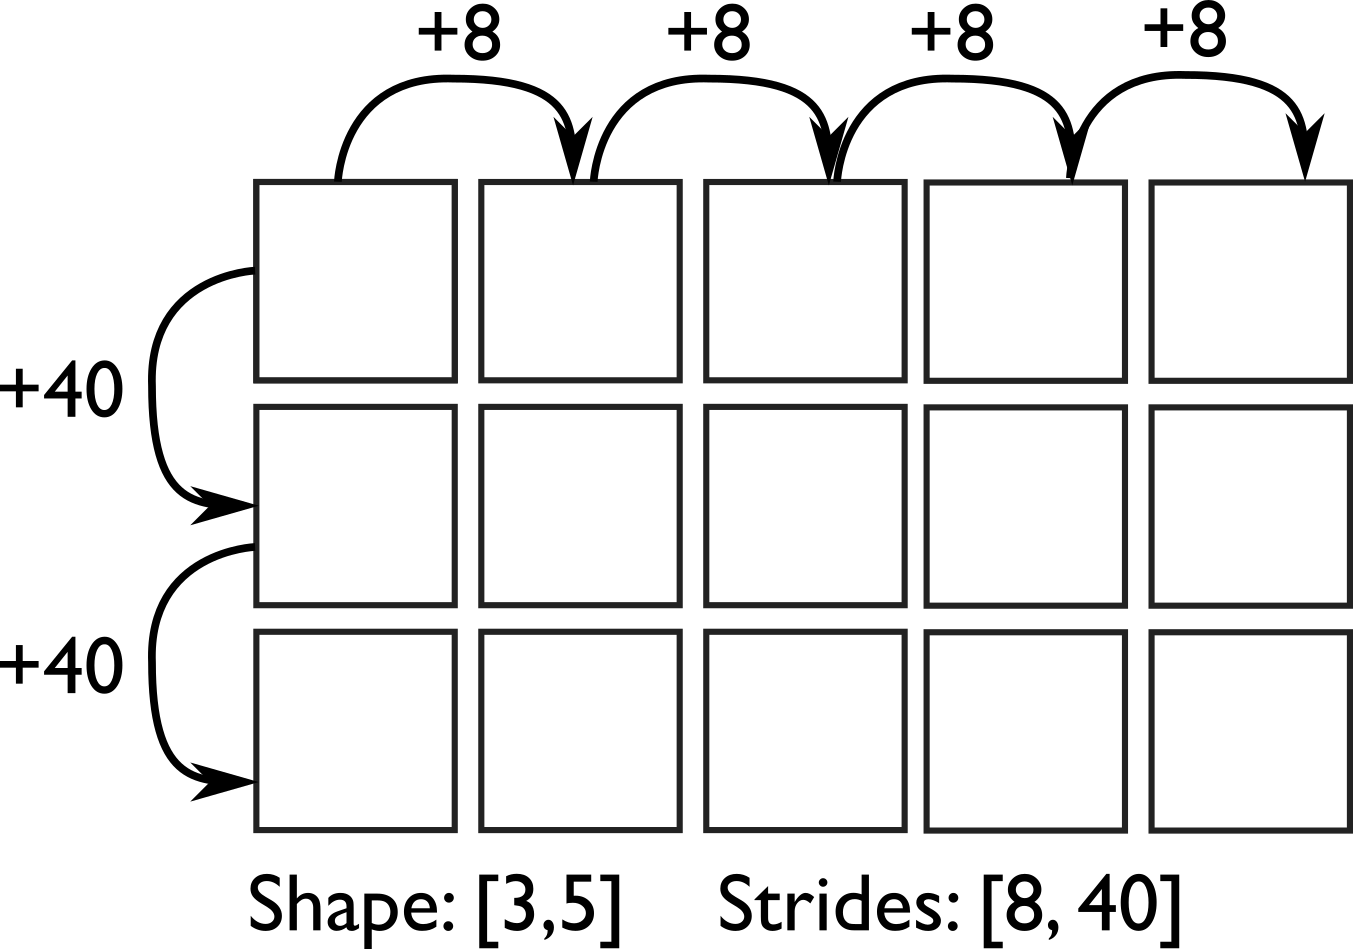
\includegraphics[scale=0.5]{src/1.4 Strides.png}
        \caption{Strides for an ndarray of shape \texttt{(3, 5)} where an element takes 8 bytes}
    \end{figure}

    In general, to find the array element at index \texttt{[i, j]} in a 2D matrix, the memory offset from the start of the number block will be:
    \[\texttt{i} * \texttt{stride[0]} + \texttt{j} * \texttt{stride[1]}.\]
    This generalises to higher dimensions (e.g. 3D, 4D tensors). To iterate through an array, the computations can simply increment by the appropriate stride to move to the next element.

    This representation of arrays is called a dope vector, which refers to the information in the strides. It is separate to the data, and part of the header. For example, the following is a \texttt{float64} 2D matrix of shape \texttt{(6, 5)}.
    \begin{table}[H]
        \centering
        \begin{tabular}{|c|c|}
            \hline
            Shape & \texttt{(6, 5)} \\
            \hline
            Strides & \texttt{(40, 8)} \\
            \hline
            Data Type & \texttt{float64} \\
            \hline
            Elements & \texttt{30} \\
            \hline
            Number of Bytes & \texttt{240} \\
            \hline
            Bits per element & \texttt{64} \\
            \hline
            Start Offset & \texttt{0} \\
            \hline
        \end{tabular}
    \end{table}
    \noindent To move to the next row, we move by $40 = 8 \times 5$ bytes, while we move to the next column, we move by 8 bytes.

    Using strides, transposition becomes $O(1)$. This is because we merely change the strides (the dope vector) and the shape. So, the transposition of the matrix above has the following shape:
    \begin{table}[H]
        \centering
        \begin{tabular}{|c|c|}
            \hline
            Shape & \texttt{(5, 6)} \\
            \hline
            Strides & \texttt{(8, 40)} \\
            \hline
            Data Type & \texttt{float64} \\
            \hline
            Elements & \texttt{30} \\
            \hline
            Number of Bytes & \texttt{240} \\
            \hline
            Bits per element & \texttt{64} \\
            \hline
            Start Offset & \texttt{0} \\
            \hline
        \end{tabular}
    \end{table}
    \noindent So, to move to the next row, instead of moving by 40 bytes, we just move by 8 in the transpose. Similarly, to move to the next column, instead of moving by 8 bytes, we move by 40 in the transpose.

    There are other operations that change the layout of the matrix, but can performed in $O(1)$, such as:
    \begin{itemize}
        \item \texttt{np.flipup(array)}, which flips the matrix up/down. So, if we flip the $6 \times 5$ matrix, we get the following shape:
        \begin{table}[H]
            \centering
            \begin{tabular}{|c|c|}
                \hline
                Shape & \texttt{(6, 5)} \\
                \hline
                Strides & \texttt{(-40, 8)} \\
                \hline
                Data Type & \texttt{float64} \\
                \hline
                Elements & \texttt{30} \\
                \hline
                Number of Bytes & \texttt{240} \\
                \hline
                Bits per element & \texttt{64} \\
                \hline
                Start Offset & \texttt{25} \\
                \hline
            \end{tabular}
        \end{table}
        We have reversed the order of the rows. For this reason, the start offset is the $(6-1) \times 5 = 25$-th element, and moving to the next row is moving back 40 bytes.
        
        \item \texttt{np.fliplr(array)}, which flips the matrix left/right.
        \begin{table}[H]
            \centering
            \begin{tabular}{|c|c|}
                \hline
                Shape & \texttt{(6, 5)} \\
                \hline
                Strides & \texttt{(40, -8)} \\
                \hline
                Data Type & \texttt{float64} \\
                \hline
                Elements & \texttt{30} \\
                \hline
                Number of Bytes & \texttt{240} \\
                \hline
                Bits per element & \texttt{64} \\
                \hline
                Start Offset & \texttt{4} \\
                \hline
            \end{tabular}
        \end{table}
        Here, we have reversed the order of the columns here. So, the start is the 4th element (the last element in the first column), and moving to the next column is moving back 8 bytes.

        \item \texttt{np.rot90(array)}, which rotates the matrix by 90 degrees.
        \begin{table}[H]
            \centering
            \begin{tabular}{|c|c|}
                \hline
                Shape & \texttt{(5, 6)} \\
                \hline
                Strides & \texttt{(-8, 40)} \\
                \hline
                Data Type & \texttt{float64} \\
                \hline
                Elements & \texttt{30} \\
                \hline
                Number of Bytes & \texttt{240} \\
                \hline
                Bits per element & \texttt{64} \\
                \hline
                Start Offset & \texttt{4} \\
                \hline
            \end{tabular}
        \end{table}
        Rotation by 90 degrees is equivalent to taking the transpose after reversing the order of the columns- the shape and the strides are flipped, but the offset remains the same.
    \end{itemize}

    NumPy gives the strides of the original matrix as \texttt{(40, 8)} and not \texttt{(8, 40)}. NumPy uses C-ordering/row major, where the last index changes first. This is different to the Fortran ordering/column major, where the first index changes fastest. We can unravel an array in both ways. 
    
    % The default type of an array in NumPy is \texttt{float64}, if any floats were given, and \texttt{int32} otherwise.
    \newpage

    \section{Tensor operations}
    \subsection{Reshaping}
    Along with transposition and flips, we can also reshape an array in constant time. This just changes how the array is indexed, i.e. the strides. We cannot change the number of elements in the array by reshaping. We reshape by \texttt{array.reshape(shape)}.

    When we reshape, the following rules are obeyed:
    \begin{itemize}
        \item the number of elements in the array remains the same;
        \item the order of the elements remains the same;
        \item the last dimension changes fastest, the second last dimension changes the second fastest, and so on.
    \end{itemize}
    We can add a (singleton) dimension by indexing with \texttt{None}, i.e. \texttt{x[:, None]} transforms a 1D vector \texttt{x} into a 2D matrix with one column in each row. We can get rid of singleton dimensions using \texttt{np.squeeze}. In tensors, we can avoid listing all the indices when slicing, e.g. \texttt{x[2, :, :, :, 5]} can be written as \texttt{x[2, .., 5]}- this is called ellision.

    \subsection{Swapping and rearranging axes}
    We can rearrange axes using \texttt{np.swapaxs(array, axis1, axis2)} to swap axes \texttt{axis1} and \texttt{axis2}.        
    
    For example, consider the following representation of a $3 \times 4 \times 5$ tensor.
    \begin{table}[H]
        \centering
        \begin{tabular}{|c|c|}
            \hline
            Shape & \texttt{(3, 4, 5)} \\
            \hline
            Strides & \texttt{(160, 40, 8)} \\
            \hline
            Data Type & \texttt{float64} \\
            \hline
            Elements & \texttt{60} \\
            \hline
            Number of Bytes & \texttt{480} \\
            \hline
            Bits per element & \texttt{64} \\
            \hline
            Start Offset & \texttt{0} \\
            \hline
        \end{tabular}
    \end{table}
    \noindent If we swap axes 0 and 2, we get the following shape:
    \begin{table}[H]
        \centering
        \begin{tabular}{|c|c|}
            \hline
            Shape & \texttt{(5, 4, 3)} \\
            \hline
            Strides & \texttt{(8, 40, 160)} \\
            \hline
            Data Type & \texttt{float64} \\
            \hline
            Elements & \texttt{60} \\
            \hline
            Number of Bytes & \texttt{480} \\
            \hline
            Bits per element & \texttt{64} \\
            \hline
            Start Offset & \texttt{0} \\
            \hline
        \end{tabular}
    \end{table}
    \noindent This happens in constant time since it merely changes the strides. Reshaping uses the powering rule, i.e. last dimension pours first. However, we might not want to amend the final dimension. In that case, we swap axes, perform the operation and swap back.

    We might need to swap multiple axes in one ago. We can do this more efficiently using \texttt{np.einsum(expression, array)}, where the expression states how the axes are moved. For example, if we change the $3 \times 4 \times 5$ tensor using the einsum, expression \texttt{ijk -> kij}, we change the axes from \texttt{(0, 1, 2)} to \texttt{(2, 0, 1)}. The representation is:
    \begin{table}[H]
        \centering
        \begin{tabular}{|c|c|}
            \hline
            Shape & \texttt{(5, 3, 4)} \\
            \hline
            Strides & \texttt{(8, 160, 40)} \\
            \hline
            Data Type & \texttt{float64} \\
            \hline
            Elements & \texttt{60} \\
            \hline
            Number of Bytes & \texttt{480} \\
            \hline
            Bits per element & \texttt{64} \\
            \hline
            Start Offset & \texttt{0} \\
            \hline
        \end{tabular}
    \end{table}
    
\end{document}